%  !TeX  root  =  user_guide.tex

\chapter{QGIS Server}\label{label_qgisserver}
\index{WMS!QGIS Server}

% when the revision of a section has been finalized,
% comment out the following line:
\updatedisclaimer

QGIS Server is an open source WMS 1.3 implementation which, in addition,
implements advanced cartographic features for thematic mapping. The QGIS
Server is a FastCGI/CGI (Common Gateway Interface) application written in
C++ that works together with a webserver (e.g. Apache, Lighttpd). It is 
funded by the EU projects Orchestra, Sany and the city of Uster in 
Switzerland.

It uses QGIS as backend for the GIS logic and for map rendering. Furthermore the 
Qt library is used for graphics and for platform independent 
C++ programming. In contrast to other WMS software, the QGIS Server uses 
cartographic rules in SLD/SE as a configuration language, both for the server 
configuration and for the user-defined cartographic rules. 

Moreover, the QGIS Server project provides the 'Publish to Web' plugin, a 
plugin for QGIS desktop which exports the current layers and symbology as a 
web project for QGIS Server (containing cartographic visualisation rules 
expressed in SLD).

As QGIS desktop and QGIS Server use the same visualization libraries, the
maps that are published on the web look the same as in desktop GIS. The 
Publish to Web plugin currently supports basic symbolization, with more complex 
cartographic visualisation rules introduced manually. As the configuration is 
performed with the SLD standard and its documented extensions, there is only 
one standardised language to learn, which greatly simplifies the complexity 
of creating maps for the Web.

In one of the following manuals we will provide a sample configuration to 
set up a QGIS Server. But for now we recommend to read one of the following 
URLs to get more information:

\begin{itemize}
\item \url{http://karlinapp.ethz.ch/qgis\_wms/} \\
\item \url{http://www.qgis.org/wiki/QGIS\_mapserver\_tutorial} \\
\item \url{http://linfiniti.com/2010/08/qgis-mapserver-a-wms-server-for-the-masses/}
\end{itemize}

\section{Sample installation on Debian Squeeze}

At this point we will give a short and simple sample installation howto for 
Debian Squeeze. Many other OS provide packages for QGIS Server, too. If you 
have to build it all from source, please refer to the URLs above.

Apart from qgis and qgis-mapserver you need a webserver, in our case apache2. 
You can install all packages with aptitude or apt-get install together 
with other necessary dependency packages.

After installation you should test, if the webserver and qgis server works as 
expected. 

Make sure the apache server is runnung with '/etc/init.d/apache2 start'. Open 
a web browser and type URL: http://localhost. If apache is up, you should see 
the message 'It works!'.

Now we test the qgis server installation. The qgis\_mapserv.fcgi is available at 
/usr/lib/cgi-bin/qgis\_mapserv.fcgi and provides a standard wms that shows the 
state boundaries of the Unites States of America \ref{fig:usa_wms}. Add 
the WMS with the URL http://localhost/cgi-bin/qgis\_mapserv.fcgi as described 
in section \ref{sec:ogc-wms-servers}.

\begin{figure}[ht]
\centering
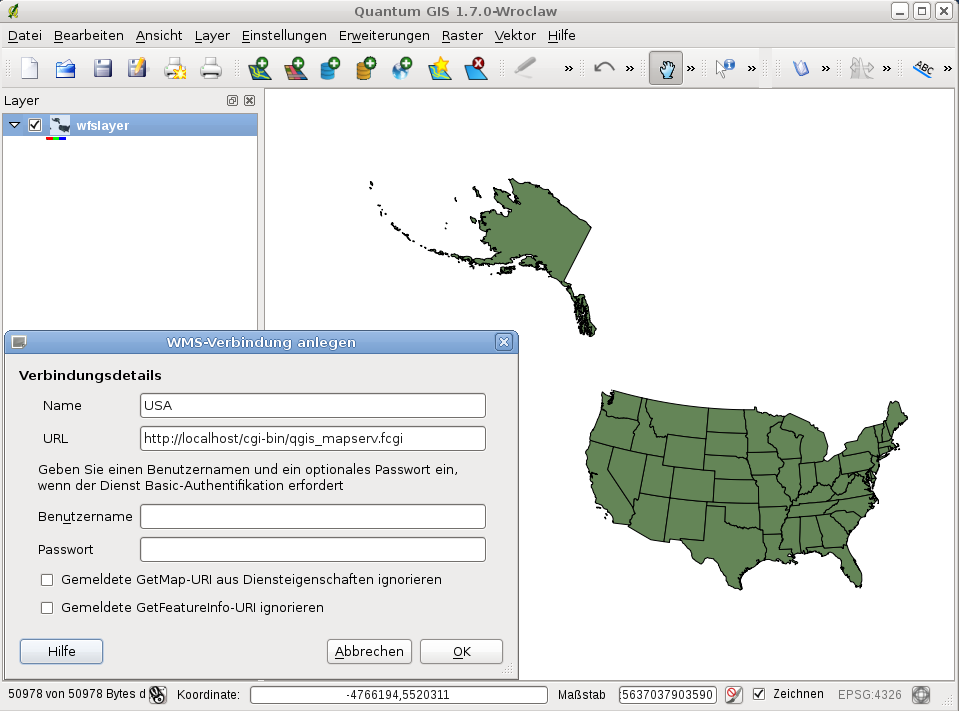
\includegraphics[clip=true, width=9cm]{standard_wms_usa}
\caption{Standard WMS with USA boundaries included in the qgis server \nixcaption}
\label{fig:usa_wms}
\end{figure}

\section{Creating a WMS from a QGIS project}

To provide a new qgis wms server we have to create a qgis project file with some 
data. Here we use the 'regions' and the 'aiport' shapefiles from the 
qgis\_sample\_dataset. 

First load the shapefiles and define the colors and styles of the layers in 
QGIS and define the project CRS, if not already done. In a next step open the 
\tab{WMS Server} tab under \mainmenuopt{Settings} \arrow \mainmenuopt{Project 
Properties} and define the fields 'Service Capabilities', 'Coordinate System 
Restrictions' and 'Advertised Extend'. Additionally you can enable the checkbox 
\checkbox{Add WKT geometry to feature into response} to make the layers 
queryable (see figure \ref{fig:wmsdefinition}). Now save the session in a 
project file 'alaska\_airports.qgs'. 

\begin{figure}[ht]
\centering
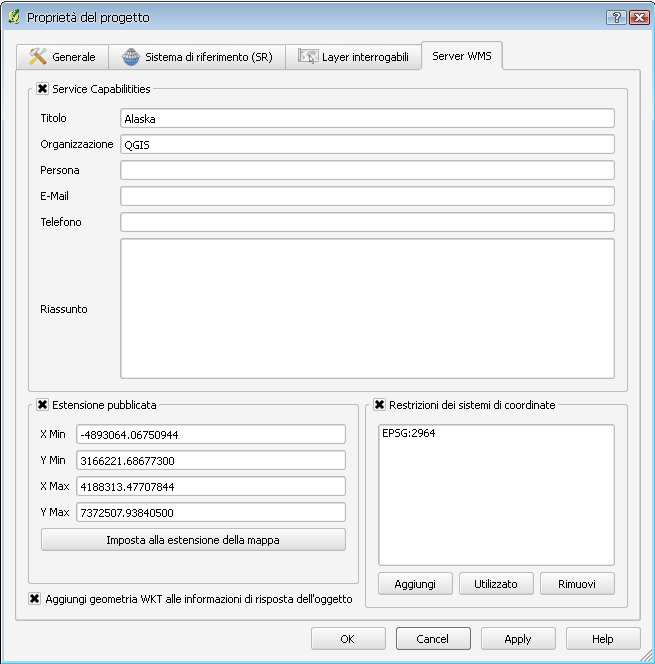
\includegraphics[clip=true, width=9cm]{wms_server_definition}
\caption{Definitions for a qgis project WMS server \nixcaption}
\label{fig:wmsdefinition}
\end{figure}

To provide the project as a WMS, we create a new folder '/usr/lib/cgi-bin/project' 
with admin privileges and add the project file 'alaska\_airports.qgs' and a copy 
of the qgis\_mapserv.fcgi file - that's all.

Now we test our project WMS, add the WMS with the URL 
http://localhost/cgi-bin/project/qgis\_mapserv.fcgi as described in section 
\ref{sec:ogc-wms-servers} to QGIS and load the WMS, see figure 
\ref{fig:wmsproject}.

\begin{figure}[ht]
\centering
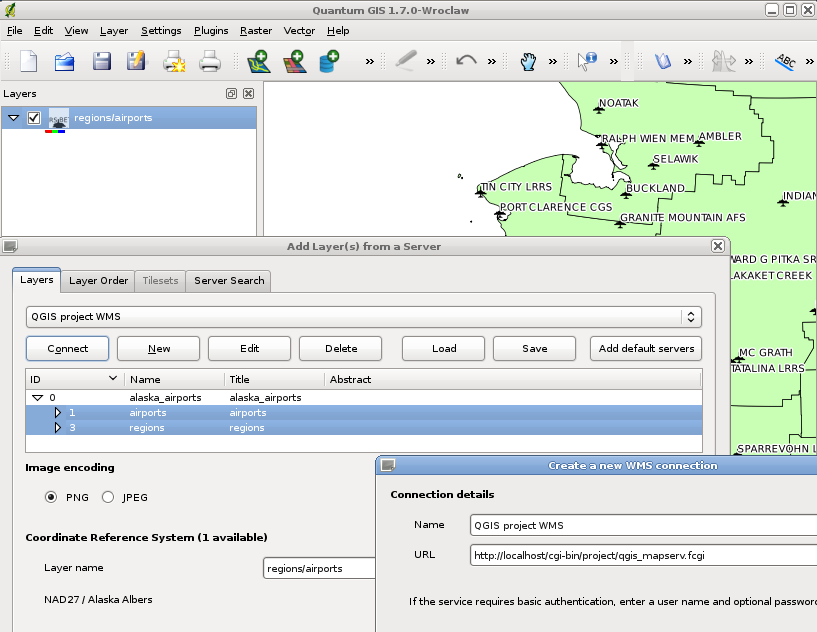
\includegraphics[clip=true, width=\textwidth]{wms_server_project}
\caption{QGIS WMS Server based on a qgis project \nixcaption}
\label{fig:wmsproject}
\end{figure}

\FloatBarrier
